\section{Finite Element Methods and Parameterised PDEs}

FEM is a numerical approach for solving PDEs by dividing the problem domain into smaller elements. Within each element, the solution is approximated using piecewise polynomial functions, forming a mesh that covers the entire domain. To solve the PDE, the weak formulation is used, which involves multiplying the PDE by a test function and integrating it over the domain. This process converts the PDE into an equivalent variational problem, simplifying the solution process, especially for problems with complex boundary conditions or irregular geometries.

Meanwhile, we are also interested in using the mixed formulation for the Poisson equation. This is a problem of interest to be developed in the NN. The mixed formulation introduces a vector variable to represent the gradient of the scalar unknown, namely the (negative) flux, leading to the new PDE:

\begin{equation*}
    -\nabla^2 u = - \nabla \sigma = f \quad \text{in }\Omega
\end{equation*}

Subject to the new Neumann boundary condition:
\begin{equation*}
    \sigma  \cdot n = g \quad \text{on }\Gamma_{N}
\end{equation*}

In solving a PDE using FEniCSx, there are three types of input parameters as mentioned previously: materials, boundary conditions, and the geometric parameter. A well-defined geometry is crucial as it directly affects the accuracy, stability, and efficiency of numerical solutions. The most common function space is the Continuous Lagrange space, which uses piecewise polynomial functions defined on each element with continuity between adjacent elements. Listing 1 shows the example codes for defining the geometric function space of a mixed-formulation problem. In particular, we have set up a function space \textbf{V}, which is created by mixing the vector and scalar elements. The vector component (flux) \textbf{Q\_el} rests on a Brezzi-Douglas-Marini (BDM) function space with a polynomial degree of k, and the scalar \textbf{P\_el} rests on the Discontinuous Galerkin (DG) space with a degree of k-1. The BDMCF space is defined on each element of the mesh and is designed to provide accurate approximations for vector quantities. The DG space allows discontinuities in the solution between neighbouring elements, making it particularly useful for problems with rapid changes or sharp gradients. 

\begin{lstlisting}[frame=single, caption={Defining geometric parameters / Creating Function Space }]
Q_el = basix.ufl.element("BDM", domain.basix_cell(), k)
P_el = basix.ufl.element("DG", domain.basix_cell(), k - 1)
V_el = basix.ufl.mixed_element([Q_el, P_el])
V = fem.functionspace(domain, V_el)
\end{lstlisting}

The materials parameters intuitively refer to the varying material properties in the problem. However, it can also extend to any parameter defining specific properties of the system, Currently, the project work is being focused on a mixed formulation of the following 2D form with five parameters $\mu_i, \text{where } i \in \{1, 2, 3, 4, 5\}$: 

\begin{align}
    u = 0 \quad & {\rm on} \ \Gamma_{D} = \{(0, y) \cup (1, y) \in \partial \Omega\} \label{bc} \\
    \text{Flux: }  g = & \sin(\mu_1 x)  \quad {\rm on} \ \Gamma_{N} = \{(x, 0) \cup (x, 1) \in \partial \Omega\} \label{flux} \\   
    \text{Source: } f & = \mu_2 \, exp\{-\mu_3[(x-\mu_4)^2 + (y-\mu_5)^2]\}  \label{source}
\end{align}

In particular, Equations \ref{bc} and \ref{flux} specify the boundary conditions of the problem, where the flux exhibits a sine wave pattern at the top and bottom, while the function u is constrained to zero at the left and right boundaries.
Equation \ref{source} defines the behaviour of the source.

The impact of different parameters is explored. Figure \ref{fig: base} shows the base case for comparison where the parameters are set to be $\bm{\mu} = [5; 10.0; 50.0; 0.5; 0.5]$.

\begin{figure}[!h]
        \begin{center}
	\begin{subfigure}{0.35\linewidth}
		\centering
		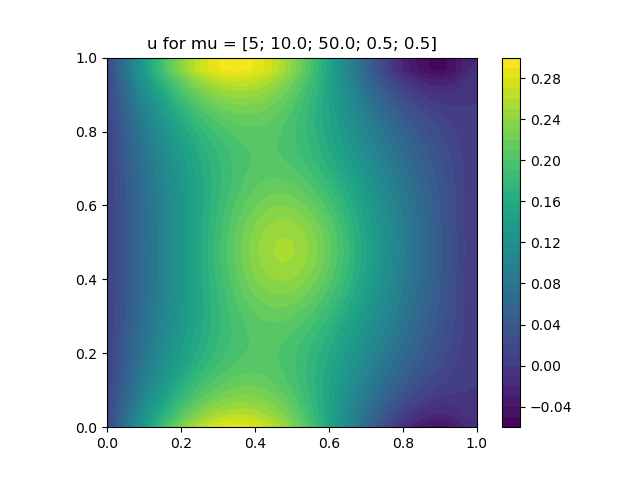
\includegraphics[width=\linewidth]{figs/mixed_u_base.png}
            \caption{base case u}
		\label{fig: base_u}
	\end{subfigure}
	\begin{subfigure}{0.35\linewidth}
		\centering
		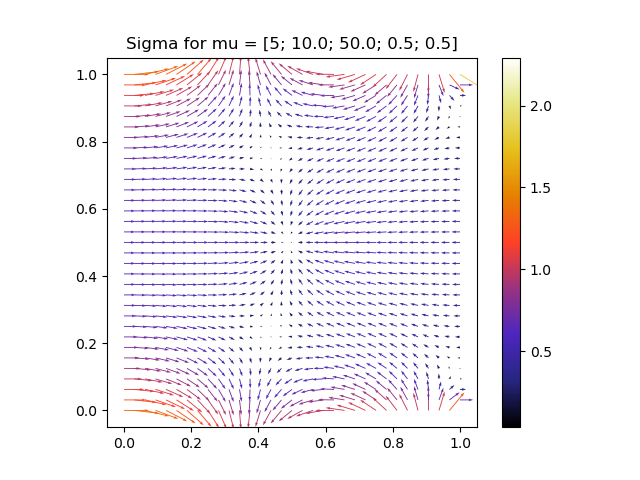
\includegraphics[width=\linewidth]{figs/mixed_sigma_base.png}
            \caption{base case $\sigma$}
		\label{fig: base_sig}
	\end{subfigure}
	\caption{Base case solutions for $\bm{\mu} = [5; 10.0; 50.0; 0.5; 0.5]$}
	\label{fig: base}
        \end{center}
\end{figure}
\begin{figure}[!htb]
    \centering
    
    \begin{subfigure}{0.35\linewidth}
        \centering
        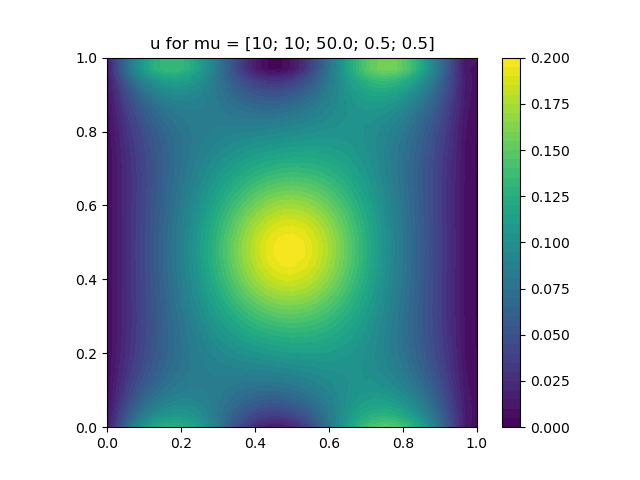
\includegraphics[width=\linewidth]{figs/mixed_u_mu11.png}
        \subcaption{Solution for u,  $\mu_1 = 10$}
        \label{subfig:mu11_a}
    \end{subfigure}%
    \begin{subfigure}{0.35\linewidth}
        \centering
        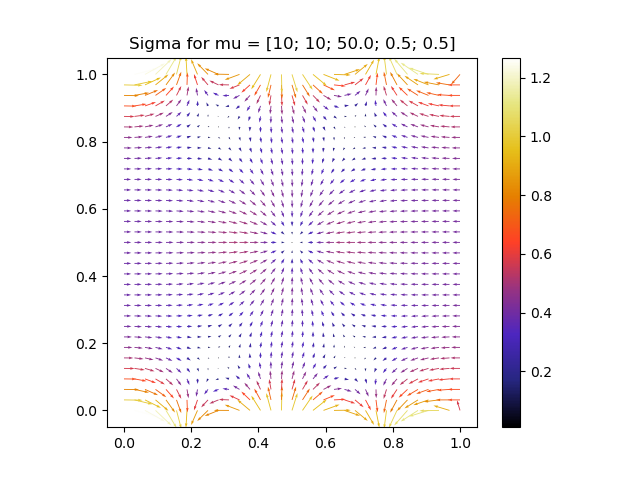
\includegraphics[width=\linewidth]{figs/mixed_sig_mu11.png}
        \subcaption{Solution for $\sigma$ , $\mu_1 = 10$}
        \label{subfig:mu11_b}
    \end{subfigure}%
    \begin{subfigure}{0.35\linewidth}
        \centering
        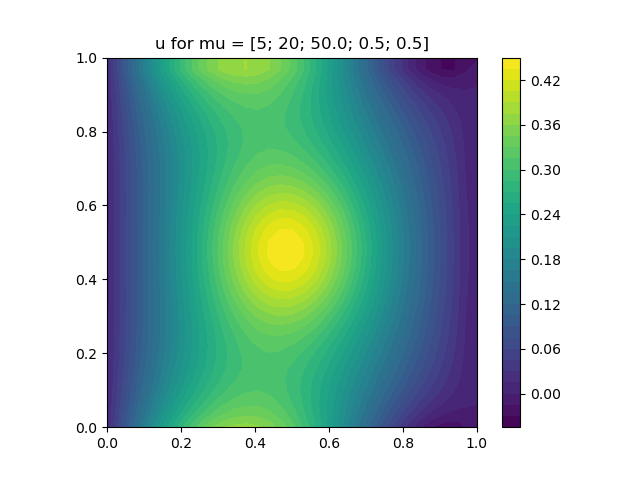
\includegraphics[width=\linewidth]{figs/mixed_u2_mu2.png}
        \subcaption{Solution for u, $\mu_2 = 20$}
        \label{subfig:mu2_a}
    \end{subfigure}
    \begin{subfigure}{0.35\linewidth}
        \centering
        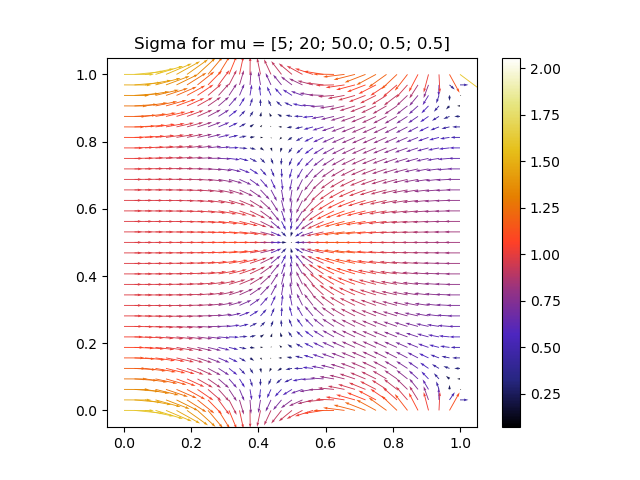
\includegraphics[width=\linewidth]{figs/mixed_sigma2_mu2.png}
        \subcaption{Solution for $\sigma$ ,$\mu_2 = 20$}
        \label{subfig:mu2_b}
    \end{subfigure}%
    \begin{subfigure}{0.35\linewidth}
        \centering
        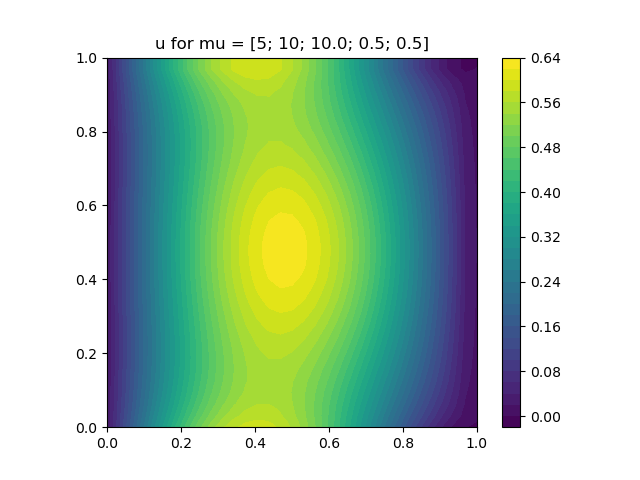
\includegraphics[width=\linewidth]{figs/mixed_u_mu3.png}
        \subcaption{Solution for u, $\mu_3 = 10$}
        \label{subfig:mu3_a}
    \end{subfigure}%
    \begin{subfigure}{0.35\linewidth}
        \centering
        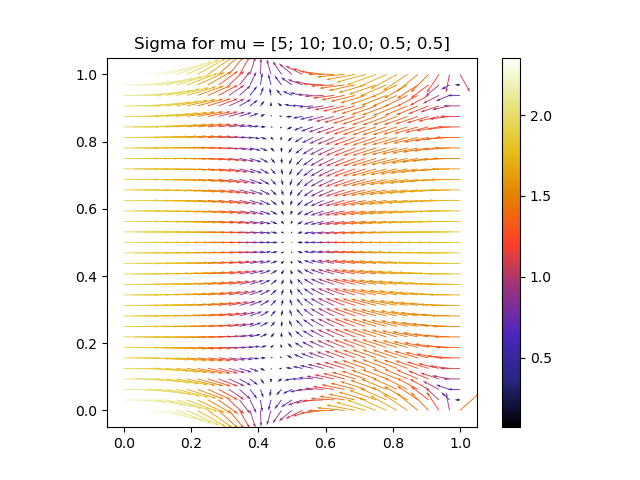
\includegraphics[width=\linewidth]{figs/mixed_sig_mu3.png}
        \subcaption{Solution for $\sigma$ , $\mu_3 = 10$}
        \label{subfig:mu3_b}
    \end{subfigure}
    \begin{subfigure}{0.4\linewidth}
        \centering
        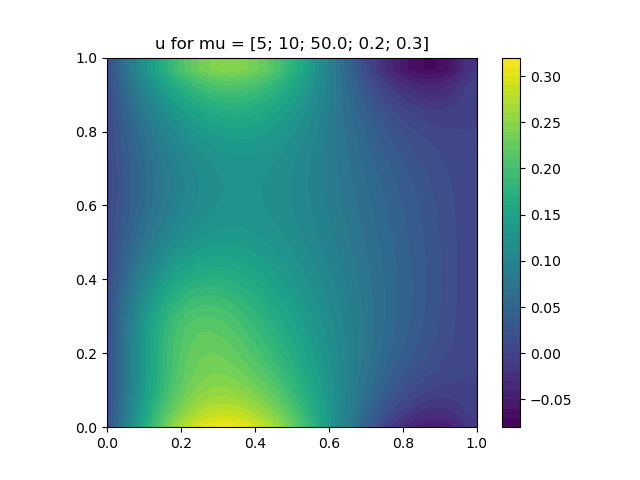
\includegraphics[width=\linewidth]{figs/mixed_u_mu45.png}
        \subcaption{Solution for u, $\mu_4, \mu_5 = 0.2, 0.3$}
        \label{subfig:mu45_a}
    \end{subfigure}
    \begin{subfigure}{0.4\linewidth}
        \centering
        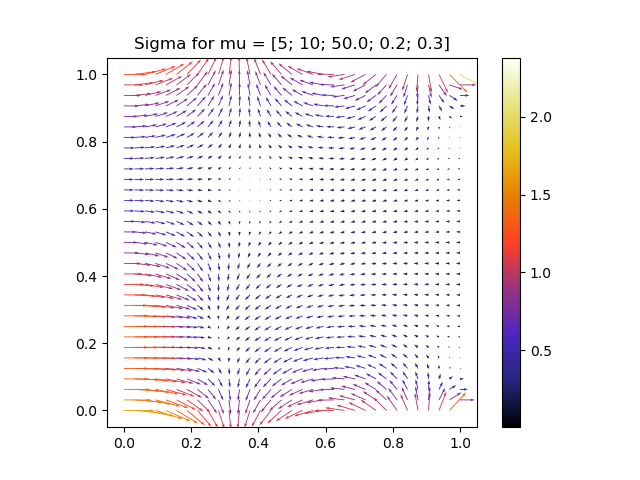
\includegraphics[width=\linewidth]{figs/mixed_sig_mu45.png}
        \subcaption{Solution for $\sigma$ , $\mu_4, \mu_5 = 0.2, 0.3$}
        \label{subfig:mu45_b}
    \end{subfigure}
    
    \caption{Solutions for different parameter variations with base case $\bm{\mu} = [5; 10.0; 50.0; 0.5; 0.5]$}
    \label{fig:all_solutions}
\end{figure}

Solutions are then compared with different initialisations of $\mu_i$, and the following were discovered based on plots varying different parameters in figure \ref{fig:all_solutions}:

\begin{itemize}
    \item $\mu_1$ controls the frequency of the flux boundary. Larger $\mu_1$ leads to a higher changing flux at the boundary, and hence more changes are imposed on u around the flux boundary.   
    \item $\mu_2$ scales the overall amplitude of u. For larger $\mu_2$, u is greater everywhere while the pattern stays the same. However, the flux would increase, especially in between the source and the boundary, where u = 0 is fixed. 
    \item $\mu_3$ controls the decay rate of the propagation of u from the source. For smaller $\mu_3$ , u is larger in unconstrained regions. However, since the boundary condition for u is fixed at 0, the flux also becomes bigger at some regions near the boundary, counterfeiting the effect of smaller decay.  
    \item $\mu_4$ and $\mu_5$ simply control the source position, whilst keeping everything else the same. Of course, the u and flux would also change accordingly. 

\end{itemize}

The problem is defined and solved with code listing 2, where a LinearProblem object that brings everything together is created. \textit{a} and \textit{L} define the weak form of the PDE, \textit{bcs} includes the functions defining the boundary conditions. Special attention is drawn to the \textit{petsc\_options}, which specifies that the LU decomposition is used as a linear solver. The choice of solvers significantly impacts the efficiency and accuracy of solving linear systems in finite element simulations. Direct solvers like the LU decomposition in this case provide accurate solutions for smaller systems but may become computationally expensive as the problem size increases. Iterative solvers are also commonly found, examples include the Conjugate Gradient (CG) or Generalized Minimal Residual (GMRES). They are suitable for large, sparse linear systems, but they are usually more complicated and require pre-conditioning to improve convergence. There are also non-linear solvers such as Newton's solver for solving non-linear PDEs. The choice of solvers is important and often involves a trade-off between accuracy and computational cost.

\begin{lstlisting}[frame=single, caption={Defining and solving the porblem}]
problem = fem.petsc.LinearProblem(a, L, bcs=bcs, \
    petsc_options={"ksp_type": "preonly", "pc_type": "lu"})
w_h = problem.solve()   # solution manifold containing u and sigma
\end{lstlisting}

In later stages, as the scale of the problems increases, more intricate conditions may arise, posing challenges for computational efficiency when utilizing FEniCSx solutions. When transitioning to the neural network (NN) approach in the future, our investigation will extend to evaluating the effectiveness of employing distinct neural networks for the flux $\sigma$ and the field $u$, as well as exploring the performance of a hyperparameter-sharing NN where the $\sigma$ and $u$ are predicted from the same NN (both after MOR with reduced basis).



